\section{Resultados e discussões}

\subsection{Pipocas e distribuição normal}
O tabuleiro teve como resultado as bolinhas se distribuindo de maneira muito similar ao desenho de sino (mais conhecido como curva normal) nas diferentes colunas, conforme evidenciado na \cref{distbolinha}. O som de pipocas estourando foi aberto no Audacity para visualizar os picos de áudio. Primeiro, o áudio foi analisado para determinar quais picos eram decorrentes de estouros de pipoca. Então, a cada trecho de 5 segundos foram contados os picos de áudio. Por fim, os dados foram plotados no gráfico representado na \cref{estouros}. A quantidade de pipocas contadas no histograma (318) diverge da quantidade contada durante o experimento (331) devido a metodologia de contagem do histograma, visto que provavelmente há picos de áudio que representam múltiplas pipocas estourando ao mesmo tempo. 

\begin{figure}[H]
    \centering
    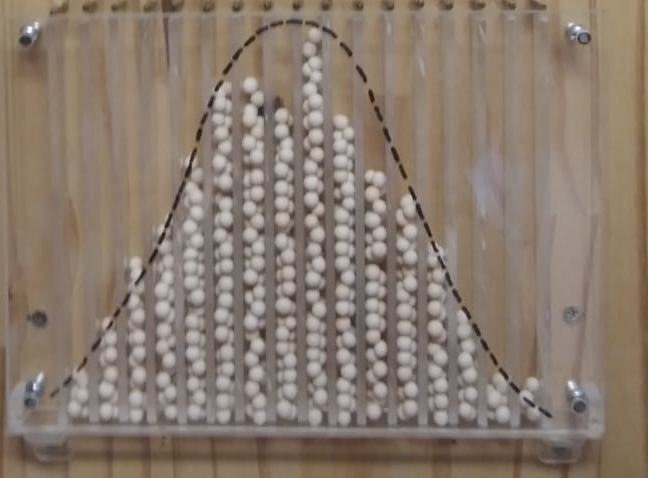
\includegraphics[width=.5\linewidth]{fig/DistNorm}
    \caption{Distribuição das bolinhas pelo tabuleiro de Galton.}\label{distbolinha}
\end{figure}
\begin{figure}[H]
    \centering
    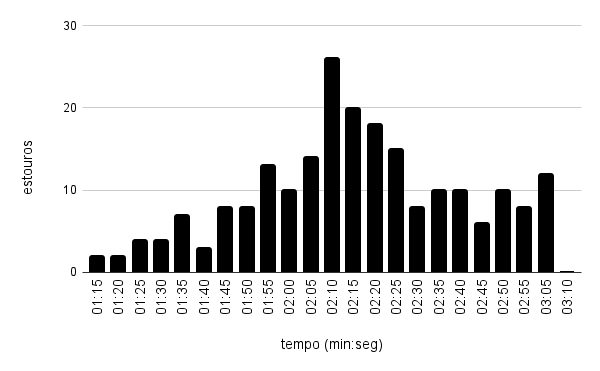
\includegraphics[width=.5\linewidth]{fig/distEstouros}
    \caption{Distribuição da quantidade de estouros por intervalos discretos de 5 em 5 segundos de tempo.}\label{estouros}
\end{figure}

É notável que a curva descrita pela \cref{estouros} se assemelha muito à de \cref{distbolinha}, porém o gráfico de estouros parece não seguir exatamente a curva de sino do lado direito e há uma boa razão para isto. Ambos os experimentos demonstram a padrões estatísticos a partir de sistemas com grande número de componentes, porém há uma diferença fundamental. No caso do tabuleiro de Galton, a cada nível, cada bolinha tem chance de ser defletida para a direita ou para a esquerda. Como as chances são iguais para os dois lados, na média, a bolinha segue o caminho do meio, e o resultado final é uma distribuição normal clássica, um comportamento estatisticamente previsível a partir de múltiplos eventos aleatórios independentes.

No caso da pipoca estourando, conforme a temperatura aumenta, as moléculas de água dentro do grão ganham energia. Um milho estoura quando a energia interna do vapor atinge um limiar crítico. A distribuição da energia cinética das moléculas em um sistema térmico não segue uma curva normal, mas sim a distribuição de Maxwell-Boltzmann. Diferentemente da distribuição normal, a curva de Maxwell-Boltzmann é assimétrica, iniciando em zero e apresentando uma ``cauda'' mais longa para energias mais altas. Isso significa que, mesmo após o pico de estouros, ainda há uma probabilidade significativa de que alguns grãos atinjam a energia necessária para estourar, resultando na queda mais gradual observada no lado direito do gráfico de estouros (\cref{estouros}). A forma da curva de estouros é, portanto, um reflexo macroscópico dessa distribuição de energias.

\subsection{Pressão na garrafa}

Os dados coletados estão resumidos na \cref{massaar}.

\begin{table}[h]
    \centering
    \caption{Dados de massa e pressão na garrafa}\label{massaar}
\begin{tabular}{l c}
\toprule
Descrição & Valor\\
\midrule
Volume da garrafa & \qty{2070}{\milli\liter} \\
Massa da garrafa & \qty{64,98}{\gram}\\
Massa da garrafa com mais ar & \qty{67,41}{\gram}\\
Pressão interna na garrafa & \qty{0,92}{\kilo\gram\per\centi\meter^2}\\
Temperatura no dia\tablefootnote{Segundo previsão do tempo do Google} & \qty{21}{\celsius} \\
\bottomrule
\end{tabular}
\end{table}

Podemos aplicar a lei dos gases ideias sobre estes dados. Massa de ar medida \(m_a = 67,41 - 64,98 = 2,43 \cdot 10^{-3}\) \si{kg}, volume da garrafa \(V = 2,070\) \si{\liter}, pressão \(P = \qty{0,92}{\kilo\gram f \per\centi\meter^2} \cdot \qty{9,8}{\frac{\newton}{\kilo\gram f}}  \cdot 10^4\si{\frac{\centi\meter^2}{\meter^2}} = 90,16\si{\kilo\pascal}\), temperatura \(T = 21 + 273 = 294\si{\kelvin}\). Com todas as unidades convertidas, começamos determinando a quantidade de moléculas de ar na garrafa: \(n = m_a/m_M\), em que \(m_M\) é a massa molar. Vamos aproximar que o ar tem massa molar igual a \qty{29}{\gram\per\mole}, então, \(n = \frac{2,43}{29} = 0,0838 \si{\mole}\). Finalmente, podemos utilizar estes valores na equação dos gases ideais e chegar a um valor para constante dos gases ideais:

\begin{align*}
    PV &= nRT\\
    R &= \frac{PV}{nT}\\
    R &= \frac{90,16 \si{\kilo\pascal} \cdot 2,070 \si{\liter}}{0,0838 \si{\mole} \cdot 294 \si{\kelvin}}\\
    R &= 7,575 \si{\kilo\pascal\liter\per\mole\per\kelvin} 
\end{align*}

O valor determinado na literatura é de \qty{0,082}{\atm\liter\per\mole\per\kelvin} que é bem próximo do obtido. Em especial, devido a medida imprecisa de temperatura há uma boa incerteza no nosso valor obtido. Somado a isso há a incerteza dos equipamentos de medição e a aproximação da massa molar do ar.

\subsection{Equipamento de teoria cinética dos gases}

Ao ligar o equipamento, observamos que conforme a potência do motor foi aumentada, as bolinhas começaram a se agitar mais intensamente e a distância entre os dois êmbolos aumentou. Ao fixar a altura do pistão superior, segurando-o pela haste, foi possível sentir um aumento na resistência do êmbolo a permanecer no local conforme a potência do motor foi aumentada. 

Como a altura do pistão de baixo era limitada (havia uma altura mínima e uma altura máxima), então sabemos com certeza que a expansão na distância entre os êmbolos tem de ser devido ao aumento na agitação das bolinhas. Isso é precisamente o modelo utilizado na teoria cinética dos gases. Se pensarmos em cada bolinha como uma molécula de gás, o aumento na potência do motor, aumenta a energia cinética média das bolinhas o que é equivalente a pensar no aumento da temperatura de um gás. Como a energia cinética média é maior, a frequência e intensidade com que as bolinhas atingem o êmbolo superior é maior, ou seja, a maior quantidade de movimento sendo transferida para o êmbolo maior. Isso faz com que ele suba ou apresente maior resistência a ficar no mesmo lugar (caso seja segurado). Ou seja, o aumento na temperatura, gera um aumento na pressão caso o volume seja mantido constante ou um aumento no volume caso a pressão seja mantida constante. 
